
\typeout{}\typeout{If latex fails to find aiaa-tc, read the README file!}
%


\documentclass[submit]{aiaa-tc_mod}% insert '[draft]' option to show overfull boxes
\usepackage[titletoc,toc]{appendix}
\usepackage{graphicx}
\usepackage{amsmath}
\usepackage{float}
%\usepackage{extsizes}
\usepackage{gensymb}
\usepackage{titlesec}
\usepackage{algorithm2e}
\restylefloat{table}
\title{End term report}
\titleformat{\chapter}{\normalfont\huge}{\thechapter.}{20pt}{\huge}
\titleformat{\paragraph}
{\normalfont\normalsize\bfseries}{\theparagraph}{1em}{}
\titlespacing*{\paragraph}
{0pt}{3.25ex plus 1ex minus .2ex}{1.5ex plus .2ex}

 \title{ Computing the Proper Orthogonal Decomposition in Parallel : 
	 Study and Implementation}

	 \author{ Govind Gopakumar }

 % Data used by 'handcarry' option if invoked
 \AIAApapernumber{2014-15}
 \AIAAconference{Mid term report, BTech Project, Aerospace Engineering}
 

% Define commands to assure consistent treatment throughout document
\newcommand{\eqnref}[1]{(\ref{#1})}
\newcommand{\class}[1]{\texttt{#1}}
\newcommand{\package}[1]{\texttt{#1}}
\newcommand{\file}[1]{\texttt{#1}}
\newcommand{\BibTeX}{\textsc{Bib}\TeX}
\setcounter{secnumdepth}{5}

\begin{document}

%\documentclass[14pt]{extreport}% insert '[draft]' option to show overfull boxes


\section*{Abstract}
We present the end term report on our work, dealing with a parallel implementation of the Proper Orthogonal Decomposition. We outline a framework for computing the POD that improves the current tools available, and can potentially speed up processes where it is applied. We also provide an overview of the POD in general, so that a reader may view this work as a self-contained introduction to both the POD as well as a sample implementation that proves to be both fast and accurate.


\clearpage

\section*{Certificate}

It is certified that the work contained in this report, titled " Parallel Proper Orthogonal Decomposition - Study and Implementation" is original, has been carried out by \textbf{Govind Gopakumar, Roll no. 11284}, and has been under my supervision. It has been done as per the requirements of the course AE471A, titled "B. T. Project"

\bigskip
\bigskip
\bigskip
\bigskip
\bigskip
\bigskip
\bigskip
\bigskip
\bigskip
\bigskip
\bigskip
\bigskip
\bigskip
\bigskip
\bigskip
\bigskip
\bigskip
\bigskip
\bigskip
\bigskip
\bigskip
\bigskip
\bigskip
\bigskip
\bigskip
\bigskip
\bigskip
\bigskip

\noindent Prof. T. K. Sengupta,\\
High Performance Computing Laboratory\\
Department of Aerospace Engineering\\
Indian Institute of Technology Kanpur\\
Kanpur 208016

\newpage
\tableofcontents
\newpage
\listoffigures
\newpage


\section{Introduction}

This project report presents the work done as part of the requirements of the B.T. Project, for the semester 2014-15 I. The Proper Orthogonal Decomposition \cite{iiscintro} is a popular technique when it comes to dealing with large data sets. Its usage varies from general modeling of chaotic systems \cite{sirovich}, where it can be used to depict a usable picture of seemingly chaotic data, to modeling large scale turbulent flows \cite{lumley}. One aspect of this project was studying the POD so that methods to speed up may be found, and if possible, to parallelize it. Our choice of parallel architecture is NVIDIA's CUDA architecture. A lot of linear algebra can be done faster when utilizing the massive parallelism inherent in GPUs \cite{gpufactorize}. We also try and study the impact of such architecture on our computations, and Analise the running times as well as accuracy with respect to traditional methods. 
\section{Background}
\subsection{Motivation}
The study of numerical solutions to flow systems has been around for a very long time. When we deal with chaotic systems, and require accuracy of a very high order, we have to deal with large scale data. The sheer amounts of data generated make it a very tough proposition, and conventional methods of analysis fail to make sense when used. This motivates us to find alternate methods to deal with such data, and one such method is the Proper Orthogonal Decomposition. As chronicled in \cite{sirovich}, the POD was proposed and rediscovered by many scientists, e.g. Kosambi (1943), Loeve (1945), Karhunen (1946). A robust statistical procedure, the POD provides us a method to approximate large data sets with a relatively lower number of dimensions. This significantly reduces our computational time, and provides more room for independent analysis. 

The POD is also an attractive procedure because of its linearity. The mathematical theory behind it is robust, and it is a safe option when applicable. This is also a potential pitfall, as computing the POD, in general, does not necessarily imply that an actual physical entity manifests itself in our analysis. It is possible to read too much into the relationships that we find using the POD, and care must be taken in our interpretation of the results obtained. 
\clearpage
\subsection{Applications}
A general procedure to reducing dimensionality, the POD is widely used across fields in statistics, computer science, signal processing, and computational fluid mechanics. An overview of the applications of the POD is provided in \cite{podintro}. A related procedure, the Principal Components Analysis \cite{googleintro} is popular among machine learning enthusiasts, used widely as a means of dealing with data too large to fit in memory, or too large to process by current means. 

While \cite{sirovich} introduced the POD as a method for dealing with large scale chaotic systems, further work has been done in adapting this procedure to the theory of mechanical systems \cite{belgium}, for reduced order modeling \cite{mit}, as well as for large data processing \cite{largedatasets}. 


In the context of turbulent flows, \cite{rowley} provides a detailed overview of the field, and the applicability of the POD. Specifically, POD was used in \cite{seng1, seng2, seng3, seng4} either as a data processing step, or as a method of obtaining better and more accurate results. 

We must take care of the fact that the POD is useful only in certain cases. As can be seen from the theory behind the POD, the lower dimension approximate is useful only in case of a high amount of correlation between some of the dimensions. In case we deal with independent dimensions, which show very little dependence on each other, we may encounter significant loss in accuracy when we obtain a lower order approximate. The POD is a tool to be used only when we can identify potential; applied blindly, it may give us results that we do not desire, and which is potentially inaccurate. 

\subsection{Theory}
\subsubsection{Proper Orthogonal Decomposition}
\paragraph{Overview of POD}
The POD is mathematically defined as an orthogonal linear transformation. We obtain a new coordinate system for our data, with the property that the greatest variance of the data, by our projection, comes to lie on the first coordinate, the second greatest variance on the second, and so on. The idea here is to choose a set of basis vectors such that the first such basis vector captures most of the variance in our data, and subsequent vectors capture decreasing amounts of variance.

With this definition, it is easy to see how the POD can be utilized in dealing with large amounts of data. If we take a dataset, and find that a large amount of the dimensions correlate with others, we can choose a combination of these as a basis vector, and approximate them to a large degree using this. 

The new set of basis vectors, and the projection of data on these vectors, prove to be uncorrelated. This allows us to ignore some of the latter vectors, which capture low amounts of variance. Ignoring a certain percentage of these basis vectors (or components), allows us to decrease the number of dimensions we deal with. 

For a more involved approach to the theory behind the POD, we would like to refer the readers to \cite{iiscintro}, which provides a rigorous explanation of why the POD works, and also provides a tutorial and sample MATLAB code for implementing the same. 

\paragraph{Computing the POD}
The idea is that, given a set of data which lies in a vector space $V$, we find a subspace $V_r$
of fixed dimension $r$ such that the error in the projection is minimized. When dealing with fluid flows,
we will assume that $V$ is essentially infinite dimensional, consisting of the values of functions on
some spatial domain. We assume that the equations or data has been discretized in space, so that $V$ has
finite dimension (for finite difference, this would be the number of grid points times number of flow variables).

Suppose we have a set of data given by $x(t) \in R^n$ with $0 \leq t \leq T $. We seek a projection
$P_r : R^n \rightarrow R^r$ that minimises the total error \\

\begin{equation}
\int_0^T (||x(t) - P_r x(t)||)^2dt 
\label{pod:1}
\end{equation}

To solve this problem, we introduce the n x n matrix : 

\begin{equation}
R = \int_0^Tx(t)x(t)^*dt
\label{pod:2}
\end{equation}

where * denotes the transpose, and find the eigenvalues and eigen vectors of R, given by,

\begin{equation}
R\phi_k = \lambda_k \phi_k, \lambda_1 \geq \dots \geq \lambda_n \geq 0
\label{pod:3}
\end{equation}

Since R is symmetric, positive-semidefinite, all the eigenvalues $\lambda_k$ are real and 
non-negative. The eigen values may be chosen to be orthonormal. This gives us an optimal 
subspace spanned by ${\phi_1, \dots, \phi_r}$ and the optimal projection given by:

\begin{equation}
P_r = \sum_{k=1}^r \phi_k \phi^*_k
\label{pod:4}
\end{equation}

The vectors $\phi_k$ are called POD modes.

\paragraph{Singular Value Decomposition}

We will also delve upon a related decomposition, namely, the Singular Value Decomposition. It is of the form : 

\begin{equation}
A = U\Sigma V^T
\label{svd:1}
\end{equation}

Where $U$ is an N x N orthogonal matrix, $\Sigma$ is an Nx M matrix which has all elements zero except along the diagonals, and $V$ is an m x m orthogonal matrix. 

The diagonal elements of $\Sigma$ consist of r=min(m,N) non-negative numbers $\sigma_i$, which are arranged in decreasing order. These are called the singular values of $A$, and are unique. The rank of $A$ determines the number of non-zero singular values it has. 


In equation \ref{svd:1}, let $U\Sigma = Q$. Then this matrix is N x m, and we can write $A = Q V^T$. Further writing it in matrix product form, we get :

\begin{equation}
A = QV^T = \sum^m_{k=1} q_k v^{T}_k
\label{svd:2}
\end{equation}

It is easy to see how this form is equivalent to what we describe in equation \ref{pod:4}.


\paragraph{Parallelizing the POD}

In popular literature, attempts have been made to parallelize the POD, but they have mainly been with the help of CPU based parallelism. \cite{alfonsi} showcases a sample implementation, and studies its performance. Although slightly outdated as far as hardware is concerned, it does show that parallelizing the POD is a promising prospect, and that the computation time can be cut down. Another work, \cite{andrecut} shows how a parallel implementation of the PCA works, but it is noted that the solution may blow up due to lack of support in hardware. A later work, \cite{iiith} implements the related decomposition, the SVD on GPUs. Again, this shows that CPU based systems are considerably outperformed by CPU based systems. 

Keeping this in mind, it is easy to attempt implementing the POD on the GPU. While certainly an exercise of great merit, it comes with its own pitfalls. Therefore, it would be advisable if, in need of a POD implementation, we use available linear algebra solutions that have proven performance on GPUs. 

\clearpage

\subsubsection{CUDA}
\paragraph{Overview}
CUDA, or Compute Unified Device Architecture, is a platform designed by NVIDIA corporation. It allows programmers to access the computational power of the GPUs present in their machines, and harness it for general purpose computation. 

\paragraph{Advantages}
GPU programming is attractive because of the following factors : 
\begin{itemize}
\item 
There are a large number of compute cores in a typical GPU as compared to a typical CPU. A low end GPU contains upwards of few hundred cores, as compared to a high end CPU which may contain less than 20 cores.

\item
These compute cores are highly interlinked and optimized for parallel execution. They are most effective when used for trivial computation that can be massively parallelized.

\item 
Looking at it from a cost-performance ratio, it is far more effective to have GPU based systems for computations. This is because a GPU will cost significantly lesser than a CPU with comparable compute power. 
\end{itemize}

\paragraph{Disadvantages}
There are certain pitfalls to using GPUs for general purpose computing. While fast and parallelizable, it is not advised to use GPUs for heavy computations. Code which needs a lot of single core computational power is ineffective when run on a GPU. Also, in case of dealing with large amounts of data, a significant overhead will be incurred in transferring the data to and from the GPU. This can be overcome by changing our program architecture to better use the inboard memory, and using CPU based computations only when necessary. 

Another aspect of GPU computing lies in the variety of GPUs available. General purpose GPUs, retailed by NVIDIA are not optimized for CUDA purposes. This results in a performance hit for most general GPUs that are available in today's machines. In case CUDA programming is the aim, care must be taken when choosing the GPU, as similar specifications but different optimizations can change results depending on our use case. 

\clearpage
\section{Methods used}
\subsection{Procedure}

As we have seen in the overview of the POD, the main step in computing the decomposition is in finding the eigenvalues of the covariance matrix. In this paper, we benchmark eigensolvers that are optimized for both CPU as well as for GPU, and contrast their performance. This allows us to show how, irrespective of the language a layman uses, the underlying implementation of the POD can be speeded up if we base it on a GPU based linear algebra system, as opposed to a CPU based system. 

We utilize the precompiled optimized binaries when comparing performance on CPUs, and use the library functions when comparing performance on GPUs. 

\subsection{Testing apparatus}

We showcase three different kinds of results, namely : 
\begin{itemize}
\item
CULA benchmarks, which have been released by the CULA authors, and compare performances between competitive CPU and GPU configurations. They utilize a computer consisting of an NVIDIA C2070 GPU and an Intel Xeon X5660 CPU running CULA R12 and Intel's MKL 10.3. The CPU benchmarks have all 6 cores active.

\item 
The computer available in HPCL, IIT Kanpur. It has an NVIDIA Quadro K2000, and an Intel Xeon E5 - 2690, running CULA R17. The benchmarking was done using precompiled binaries which use Intel MKL, and an average of 17 cores of the CPU were part of the benchmark. 

\item
A general benchmark, between Intel's MKL implementation of linear algebra routines and CULA Dense's implementation. The reference machines used are Intel Core -i7 3770, and an NVIDIA GeForce GTX580.

\end{itemize}
\subsection{Libraries used}
For this project, we use the CULA library \cite{culamain}, which provides us basic linear algebra routines. From our theoretical analysis, it is easy to see that the most time consuming and rigorous step in computing the POD of a data set is the eigenvector decomposition of our covariance matrix. This can be done effectively and fast using commercially available routines, which are highly optimized for the GPU architecture. 
\subsection{Psuedo code}
We provide below the pseudo-code used in our computation of the POD. Readers will realize that computing the POD, or at least, the basis vectors is a trivial task when broken down into elementary steps. It can be achieved in a very small number of steps utilizing commercially available software, which has been fine tuned for performance and accuracy. 

\begin{enumerate}
\item
Locate and load data set $X$, which we wish to transform into a reduced set.

\item
Initialize the CUDA environment. 

\item
Shift all the points in our dataset with respect to the mean. This is done to facilitate an easier computation of the POD coordinate system. 

\item
Compute the Covariance matrix, $P = X X^T$. This can be obtained using the matrixMul functions available in both stock CUBLAS libraries as well as the CULA library.

\item
Compute the eigenvectors, $V$ of the Covariance matrix, $P$. This can be obtained using either the SSYEV or DSYEV functions in CULA, as per required accuracy. 

\item 
The obtained set $V$, when ordered according to the associated Eigen Values, form the vectors that encompass the highest variance, the second highest variance, and so on, in order. 

\item
Choosing an orthonormal set of eigenvectors, we obtain our new coordinate system. 

\item
We can now transform the required data set using our eigenvectors, dropping the eigenvectors corresponding to lower eigenvalues, as per our requirements.
\end{enumerate}
\clearpage
\section{Results}

\subsection{CULA standard benchmarks}

The following are standard benchmarks that the authors of CULA provide. As they note, they use a comparable CPU-GPU pair, and the GPU outperforms the CPU on all possible counts. It so happens that the CPU shows better performance only with small amounts of data, and asymptotically, the performance of the GPU based systems are far better. 

\subsubsection{Performance charts - Eigenvector Decomposition}


\begin{figure}[H]
 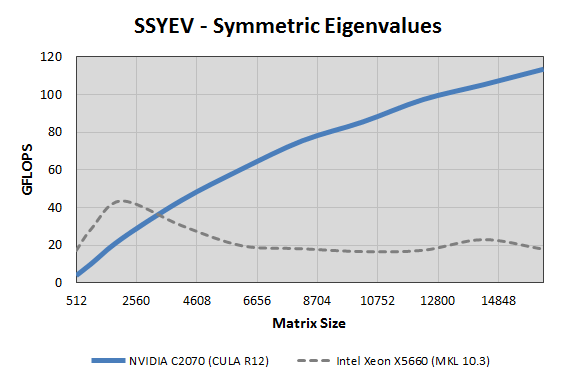
\includegraphics[width=\textwidth]{SSYEV_N.png}
 \caption{Single precision Eigenvector Decomposition - CULA}
 \label{ssyev}
\end{figure}

\begin{figure}[H]
 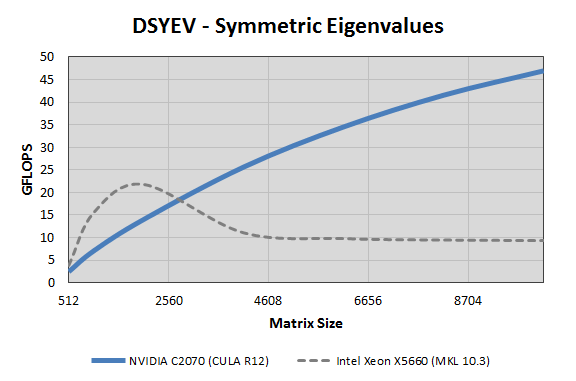
\includegraphics[width=\textwidth]{DSYEV_N.png}
 \caption{Double precision Eigenvector decomposition - CULA}
 \label{dsyev}
\end{figure}

\subsubsection{Performance charts - SVD}


\begin{figure}[H]
 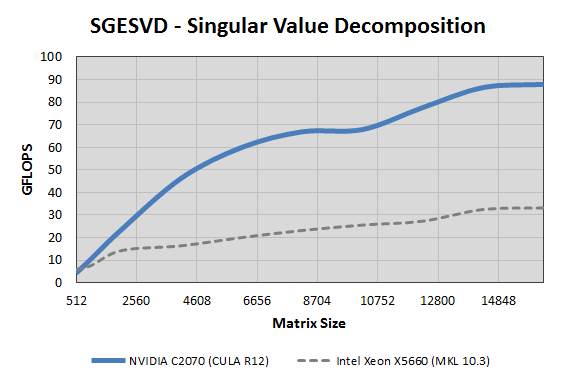
\includegraphics[width=\textwidth]{SGESVD.png}
 \caption{Single precision SVD - CULA}
 \label{sgesvd}
\end{figure}

\begin{figure}[H]
 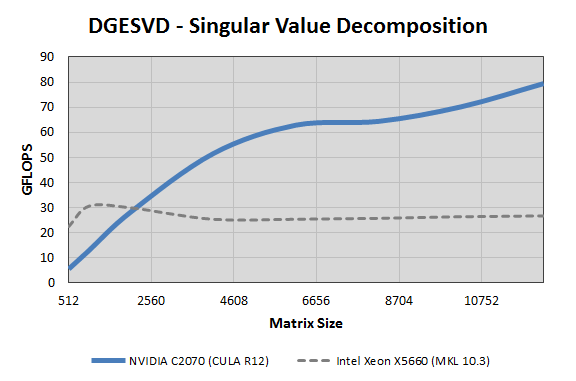
\includegraphics[width=\textwidth]{DGESVD.png}
 \caption{Double precision SVD - CULA}
 \label{dgesvd}
\end{figure}

\subsubsection{Inferences}

As we can see, the GPU based system outperforms the CPU based systems considerably. It can also be noted that when we deal with small amounts of data, the CPU is actually faster in some cases, but beyond a certain limit, the GPU always performs better then the CPU.

\subsection{HPCL benchmarks}
The HPCL computer hosts a Quadro K2000, which by design is not meant as a CUDA compute device. From our results, we can see that it generally matches the performance of the 20 core Intel Xeon CPU. Accuracy is main tainted through double precision modes in the GPU, and even in this mode, the time taken is comparable to that of the CPU. While utilizing all 20 cores of the CPU will no doubt provide an advantage, it was noted during the test that the CPU usage never dropped below 17/20. At higher amounts of data, the bandwidth of the GPU limits the computational power. This can be easily overcome if we use a GPU that is meant for CUDA computations. 

\subsubsection{Performance - SVD}
\begin{figure}[H]
 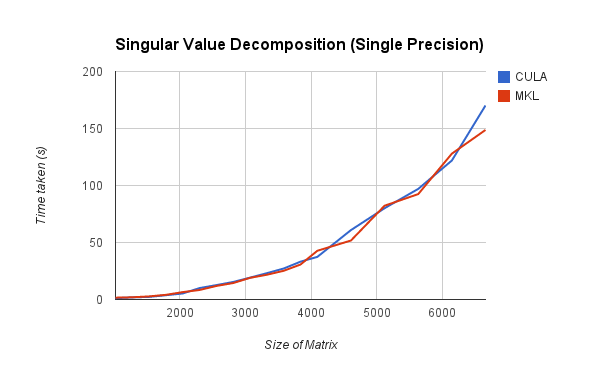
\includegraphics[width=\textwidth]{hpclsgesvd.png}
 \caption{Single precision SVD - HPCL}
 \label{hpclsgesvd}
\end{figure}

\begin{figure}[H]
 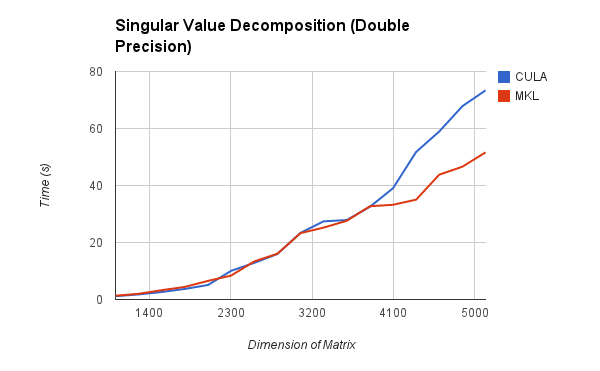
\includegraphics[width=\textwidth]{hpcldgesvd.png}
 \caption{Double precision SVD - HPCL}
 \label{hpcldgesvd}
\end{figure}

\subsubsection{Inferences}

As mentioned elsewhere in this work, the graphics card that is present in the GPU of the HPCL main machine is not meant for CUDA usage. It supports an outdated version of NVIDIA's compute drivers, and is mainly for usage in rendering and other general tasks. The CPU is a 20 core Intel Xeon machine, meant for general purpose computing, including floating point calculations. Even with this imbalance in design, the GPU performs quite close to the CPU, and loses out when presented with very large sizes, which is beyond its bandwidth capabilities. The CPU can utilize most of its cores, as well as the tremendous amount of RAM at its disposal to perform better than the GPU. 

\subsection{Benchmarking using standard configuration}

We benchmark the double precision routines using standard computing facilities, that should be available in a general computing cluster. 
\subsubsection{Independent benchmarking}

\begin{figure}[H]
 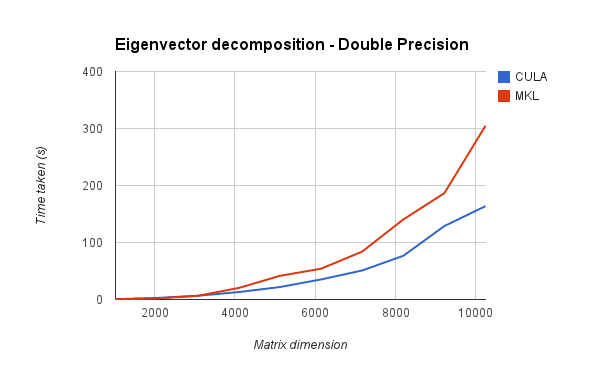
\includegraphics[width=\textwidth]{dsyev_bench.png}
 \caption{Eigenvector decomposition - Double precision benchmarks }
 \label{eigenbench}
\end{figure}

\begin{figure}[H]
 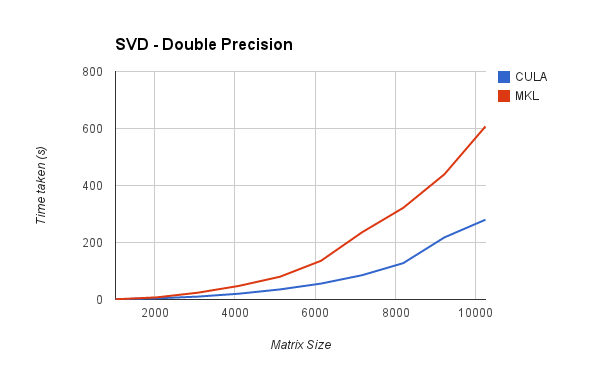
\includegraphics[width=\textwidth]{dgesvd_bench.png}
 \caption{SVD  Double precision benchmarks }
 \label{svdbench}
\end{figure}


\subsubsection{Inferences}
As we can see, independent analysis confirms what we know from published literature, that linear algebra routines are faster on the GPU, as compared to on the CPU. This particular set of results come from a comparable set of GPU-CPU pairing, which can be found as part of the facilities of a general computing cluster. This should serve as a good indicator of performance of real world GPUs.

\clearpage
\section{Conclusion}

\subsection{Remarks}
We make the following comments as regards GPU performance, as well as computing the POD :

\begin{itemize}

\item
The POD is inherently based on basic linear algebra routines. The popularity of such routines mean that a lot of optimization has been done in standard implementations, and as an end user, it is far more effective to use an existing implementation rather than trying to recreate one. 

\item
Linear algebra routines, like eigenvector decomposition and singular value decomposition can be parallelized with the help of computing architectures. Parallel implementations significantly outperform sequential implementations.

\item
GPU architectures provide a platform for much more parallelization as compared to CPU platforms. The standard CPU comes with roughly 16 cores, whereas an entry level GPU comes with a few hundred cores. 

\item
CPUs traditionally perform very well on double precision as well as single precision, whereas GPU performance on the former is worse as compared to on the latter. 

\item
Modern day GPUs outperform comparable CPUs when it comes to most linear algebra routines. This can be observed in a lot of the state of the art, and speedups can be of the order of 10 or more.

\item 
As regards the POD, it is far more efficient to switch to a GPU based compute system. As we showed in our results section, an entry level GPU could compete effectively with a high-end CPU, and at times outperformed the CPU in single precision tests. 

\item
The ease of use of GPU architectures, as well as the extensibility of libraries like CULA make a compelling case for switching over to GPU for any form of intensive computing. 
\end{itemize}

\subsection{Future work and extensions}
This report mainly focused on comparing CPU performance with GPUs, and specifically focused on how it effects our computation of the POD. While one of the secondary objectives was the implementation of the POD using GPU architectures, it was realized that this would be a straightforward procedure, and due to the variety of languages used in scientific programming, a language agnostic version implementation would be ideal. 

Future work could include the following :

\begin{itemize}
\item
Extending to a stand alone executable, which computes the POD according to user defined arguments and data. This would make it very easy for the end user to utilize this as a product, and would complement not only flow analysis, but also all other fields which use this technique.

\item
Specific to IIT Kanpur, and HPCL, this procedure can be extended as a binding to the commercial software, MATLAB. The current methods that form the underlying linear algebra systems for MATLAB utilize CPU based computations. It is an almost trivial exercise to convert this to a GPU based system, and it can speed up procedures massively. 

\item
While still in its infancy, neural networks have been shown to correlate well with learning lower dimensional projections. While the POD method creates a linear vector space, a neural network has been shown to learn even non-linear spaces into which data can be projected. This has been shown to be an efficient method of data compression in \cite{hinton}. Exploring this path might lead to some more ideas in the field of reduced order modeling. 
\end{itemize}

\clearpage
\begin{thebibliography}{20}% maximum number of references (for label width)
 \bibitem{seng1}
 Nonlinear Receptivity and Instability Studies by Proper Orthogonal Decomposition, 
 T.K. Sengupta et. al., 
 Hawaii Summer Conferences, 
 2011
 
\bibitem{seng2}
Dynamical System Approach to Instability of Flow Past a Circular Cylinder, 
T.K.Sengupta et. al., 
J. Fluid Mech., 
2010

\bibitem{seng3}
Proper Orthogonal Decomposition of Direct Numerical Simulation Data of By-pass Transition, 
T.K. Sengupta et. al., 
Computers and Structures, 
2004

\bibitem{seng4}
Universal Instability Modes in Internal and External Flows, 
T.K. Sengupta et. al., 
Computers and Fluids,
2011

\bibitem{lumley}
The Proper Orthogonal Decomposition in the Analysis of Turbulent Flows, 
Gal Berkooz et. al.,
Annu. Rev. Fluid Mech., 
1993

\bibitem{rowley}
Model Reduction for Fluids, using Balanced Proper Orthogonal Decomposition, 
C.W. Rowley, 
Int. Journal of Bifurcation and Chaos, 
2005

\bibitem{sirovich}
Chaotic Dynamics of Coherent Structures, 
L. Sirovich,
Physica D 37, 
1989

\bibitem{mit}
Balanced Model Reduction via the Proper Orthogonal Decomposition,
K. Willcox et. al., 
AIAA Journal,
2002

\bibitem{belgium}
The Method of Proper Orthogonal Decomposition for Dynamical Characterization and Order Reduction of Mechanical Systems : An Overview,
Gaetan Kerschen et. al., 
Nonlinear Dynamics, 
2005


\bibitem{largedatasets}
PCA for Large Data Sets with Parallel Data Summarization,
Carlos Ordonez et. al., 
DAPD Journal, 
2014

\bibitem{alfonsi}
A Parallel Computational Code for the Proper Orthogonal Decomposition of Turbulent Flows,
Giancarlo Alfonsi et. al., 
Journal of Flow Visualization and Image Processing, 
2007

\bibitem{googleintro}
A tutorial on Principal Component Analysis
Jonathon Shlens, 
Arxiv, 
2014


\bibitem{iiscintro}
An Introduction to the Proper Orthogonal Decomposition, 
Anindya Chatterjee, 
IISc Tutorials, 
SERC IISc

\bibitem{podintro}
Proper Orthogonal Decomposition and its Applications,
Y.C.Liang et. al., 
Journal of Sound and Vibration, 
2002

\bibitem{gpufactorize} 
LU, QR, and Cholesky Factorizations using Vector Capablities of GPUs, 
Vasily Volkov et. al., 
Technical Report UC Berkeley, 
2008

\bibitem{andrecut}
Parallel GPU Implementation of Iterative PCA Algorithms, 
M. Andrecut, 
Arxiv, 
2008

\bibitem{iiith}
Singular Value Decomposition on GPU using CUDA, 
Sheetal Lahabar et. al., 
IPDPS, 
2009

\bibitem{culamain}
CULA : Hybrid GPU Accelerated Linear Algebra Routines,
J.R.Humphrey et. al., 
SPIE DSS, 
2010

\bibitem{hinton}
Reducing the Dimensionality of Data with Neural Networks, 
G.E.Hinton et. al., 
Science, 
2006
 
\end{thebibliography}

\end{document}

% - Release $Name:  $ -